%RESULTSS

After implementing the software in the GridCal package, now it is time to test how this solver performs when compared to already available solutions. The benchmark used for this comparison will be the Matpower solver \cite{zimmerman2010matpower},
an open-source package that has been used in many works as a reference for the AC-OPF problem. The objective is to have a similar runtime and number of iterations for the base AC-OPF problem (the model already used by Matpower's solver),
and to see how well does it scale when the new features are added. 

The grids used for this benchmark are a combination of small grids with some interesting configurations that allow some testing of the new features, and larger grids that will be used to see if the solver is capable to solve them 
and what is the computational cost of doing so. The largest grid is the Great Britain national grid (an adaptation), which can give some insight on how the solver performs in a real-world scenario.

The results obtained have been obtained in a computer with the following specifications:

\begin{itemize}
    \item CPU: Intel Core i7-1165G7 @ 2.80GHz
    \item RAM: 16GB DDR4
    \item GPU: Intel Iris Xe Graphics
    \item OS: Windows 11
    \item IDE: PyCharm
    \item Python version: 3.10
    \item Matpower version - Python version: PyPower 5.1.16 \cite{zimmerman2010matpower} \cite{lincoln2023pypower}
\end{itemize}

And the tolerance requested for the convergence conditions is $10^{-6}$.

There are two possible initializations for the solver, which are the following:

\begin{itemize}
    \item \textbf{Power flow initialization:} The solver uses GridCal's built-in power flow with the default values introduced in the grid model as the initial values for the variables. The results of the power flow solver are used as the starting point for the optimization variables.
    \item \textbf{Basic initialization:} This is the initialization used by Matpower, which sets the variables at the center of the domain. Although it seems simpler, for some cases it could be better to ensure all the variables are not too close to some of their limits.
\end{itemize}

The use of bound slacks has also been tested for both initialization options, yielding a total of 4 different combinations per case. The results will be shown in the following subsections.

\subsection{Error evolution}

The first comparison carried out is the error evolution for the different cases. The graphs portray the error at each iteration for the different initialization settings, and will be compared to the error obtained by Matpower's solver. The error is the maximum value
of the expressions~\eqref{eq:conv_cond} at each iteration. This error corresponds to the maximum value of the convergence conditions, which are
calculated for each derivative of the Lagrangian, and including the $\gamma$ value. The error should always tend to decrease, although sometimes it does so really slowly, or it even goes up for some iterations. 
This could mean that the path taken by the interior point method is exceeding some limits, and the resulting new point is worse than the previous.
Excessive increases of the error are normally avoided by the step control implemented in the solver, although it does not prevent these increases in problems that are ill-conditioned or
even unsolvable.

\subsubsection{Case 9-bus}

The first case is a 9-bus system \cite{chow1982time} which can be useful to see the behavior of the algorithm in a small system, while it can be portrayed as shown in Figure~\ref{fig:case9topo} with sufficient clarity in this project using the GridCal GUI. %Insert reference


\begin{figure}[H]
  \centering
  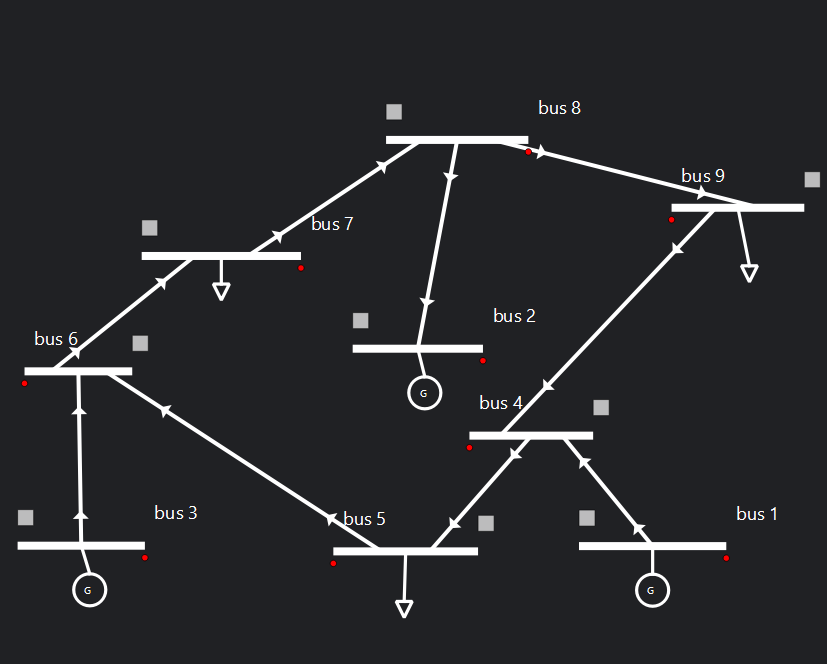
\includegraphics[width= 250 px]{Images/case9_topo.png}
  \caption{Schematic of the 9-bus grid.}
  \label{fig:case9topo}
\end{figure}

It can be seen in Figure~\ref{fig:9bus_error} that for such a small grid, there is not a significant difference between the different initialization options. The error evolution is very similar for all of them, and the error obtained is very close to the one obtained by Matpower, 
being the option without bound slacks slightly better as the vector of variables is considerably smaller. If there are no issues with the grid, the initialization with bound slacks is not necessary for this case.

\begin{figure}[!htb]
    \centering
    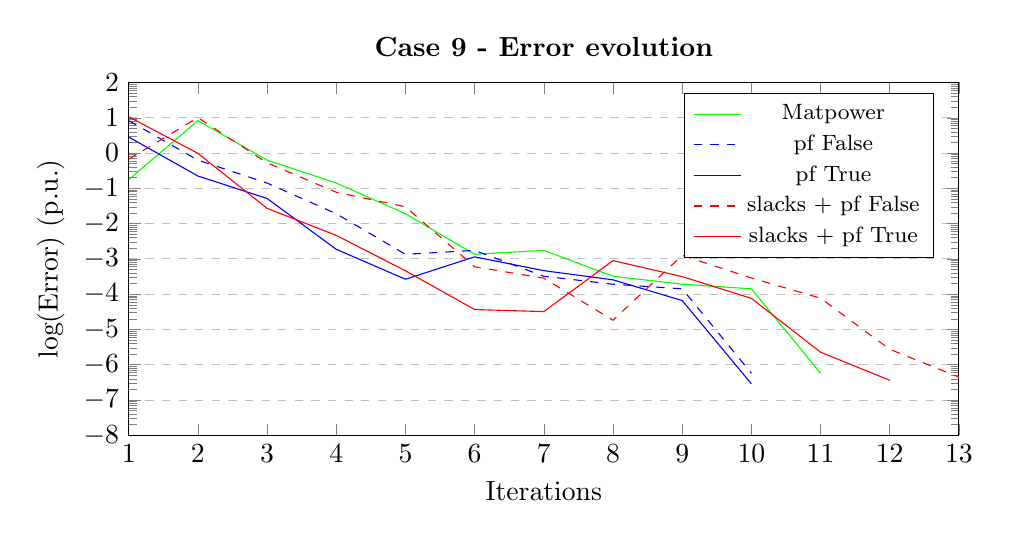
\begin{tikzpicture}
    \begin{semilogyaxis}[
        title={\textbf{Case 9 - Error evolution}},
        xlabel={Iterations},
        ylabel={log(Error) (p.u.)},
        width= \textwidth,
        height= 0.5\textwidth,
        xmin=1, xmax=13,
        ymin=1e-8, ymax=1e2,
        xtick={1,2,3,4,5,6,7,8,9,10,11,12,13},
        %ytick={1e-8,1e-6,1e-4,1e-2,1e0,1e2},
        log base 10 number format code/.code={\pgfmathprintnumber[fixed]{#1}},
        max space between ticks=20,
        legend pos=north east,
        ymajorgrids=true,
        grid style=dashed,
        scaled ticks=false,
        yticklabel style={/pgf/number format/sci},
        legend style={font=\footnotesize},        
    ]

    %Data for Matpower
    \addplot[
        color=green,
        mark=none,
        mark options={solid}
        ]
        coordinates {
        (1, 0.1765)
        (2, 8.305054238)
        (3, 0.630697772)
        (4, 0.141403676)
        (5, 0.019075407)
        (6, 0.001352357)
        (7, 0.001746417)
        (8, 0.000322236)
        (9, 0.000191987)
        (10, 0.000142097)
        (11, 5.75478E-07)
        };
        \addlegendentry{Matpower}

    % Data for 'pf False' plotted with dashed lines
    \addplot[
        color=blue,
        dashed,
        mark=none,
        mark options={dashed}
        ]
        coordinates {
        (1,8.305054238)(2,0.630697772)(3,0.141403676)(4,0.019075407)
        (5,0.001352357)(6,0.001746417)(7,0.000322236)(8,0.000191987)(9,0.000142097)
        (10,5.75e-07)
        };
        \addlegendentry{pf False}

    % Data for 'pf True'
    \addplot[
        color=blue,
        mark=none,
        mark options={solid}
        ]
        coordinates {
        (1,2.8442694)(2,0.224084957)(3,0.051708904)(4,0.001873459)
        (5,0.000265494)(6,0.001145971)(7,0.000464665)(8,0.00025553)(9,6.60e-05)
        (10,2.89e-07)
        };
        \addlegendentry{pf True}

    %Data for slacks + pf False
    \addplot[
        color=red,
        mark=none,
        dashed,
        mark options={dashed}
        ]
        coordinates {
    (1, 0.672594031)
    (2, 10.08607297)
    (3, 0.527802283)
    (4, 0.077601018)
    (5, 0.030048859)
    (6, 0.000599489)
    (7, 0.000284285)
    (8, 1.83E-05)
    (9, 0.001257839)
    (10, 0.000288391)
    (11, 7.69E-05)
    (12, 2.74E-06)
    (13, 4.47E-07)
        };
        \addlegendentry{slacks + pf False}

         %Data for slacks + pf True'
    \addplot[
        color=red,
        mark=none,
        mark options={solid}
        ]
        coordinates {
    (1, 10.69785291)
    (2, 0.981962281)
    (3, 0.027127147)
    (4, 0.004650334)
    (5, 0.000460963)
    (6, 3.68E-05)
    (7, 3.21E-05)
    (8, 0.000893703)
    (9, 0.0003156)
    (10, 7.62E-05)
    (11, 2.27E-06)
    (12, 3.64E-07)
        };
        \addlegendentry{slacks + pf True}

    \end{semilogyaxis}
    \end{tikzpicture}
    \caption{Error evolution for the Case 9 system for different initialization options.}
    \label{fig:9bus_error}
\end{figure}

The result can be visualized in GridCal's GUI as shown in Figure~\ref{fig:case9solved}.

\begin{figure}[H]
    \centering
    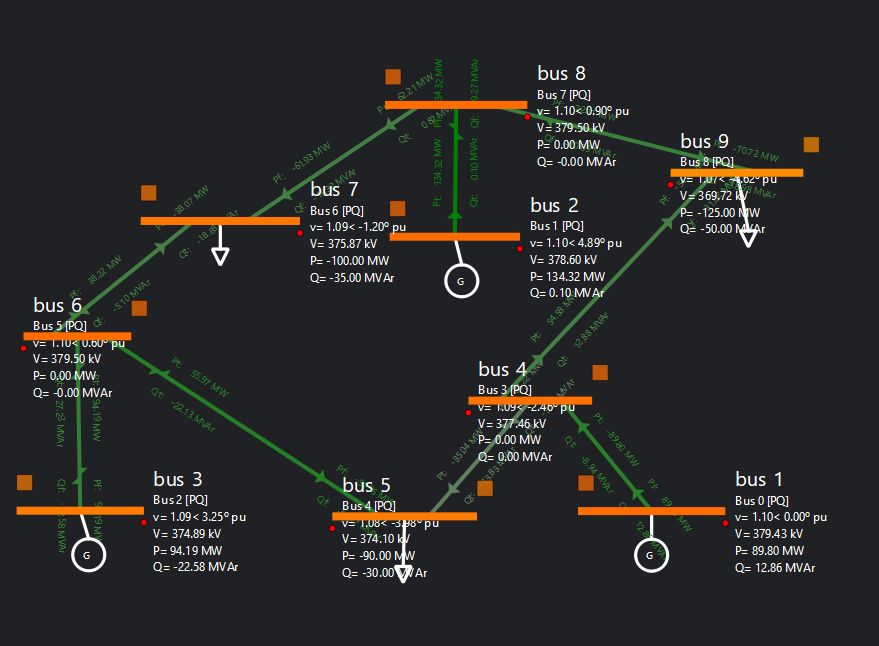
\includegraphics[width=250px]{Images/case9_solved.png}
    \caption{Plot of the solution of Case 9.}
    \label{fig:case9solved}
  \end{figure}

Something that can catch the eye is the orange color of the bus, which means they are near their upper voltage limit. This is due to the optimization trying to raise the voltage value as high as the limit allows
to reduce the current flowing through the lines, which reduces quadratically the losses. 

\subsubsection{Case Pegase89}

The next grid studied is a case with 89 buses obtained from the Pegase database \cite{josz2016ac}, with an interesting result shown in Figure~\ref{fig:peg89_error}.

%%%%%%%%%%%%%%%%%%%%%%%PEGASE89

\begin{figure}[H]
    \centering
    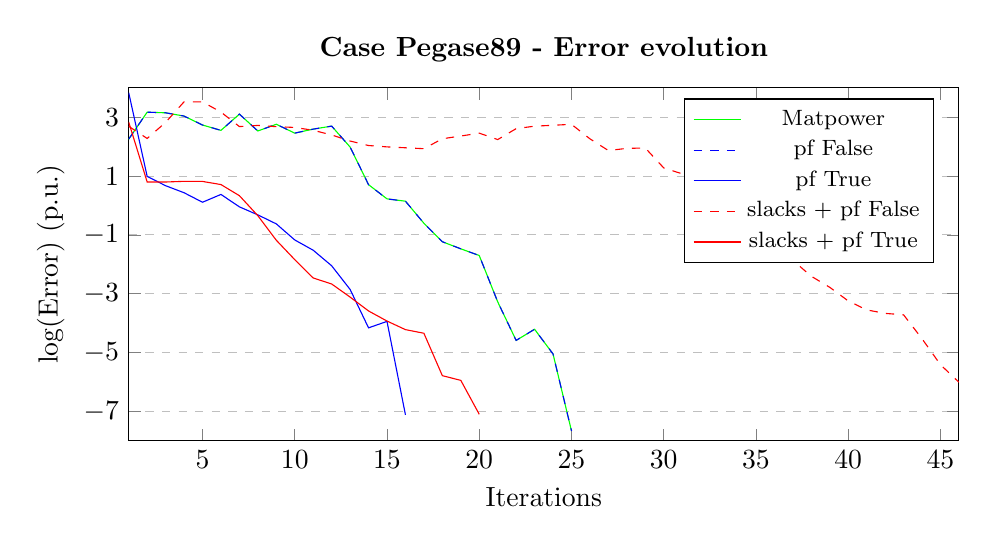
\begin{tikzpicture}
    \begin{semilogyaxis}[
        title={\textbf{Case Pegase89 - Error evolution}},
        xlabel={Iterations},
        ylabel={log(Error) (p.u.)},
        width=\textwidth,
        height=0.5\textwidth,
        xmin=1, xmax=46,
        ymin=1e-8, ymax=1e4,
        xtick={5,10,15,20,25,30,35,40,45},
        %ytick={1e-8,1e-6,1e-4,1e-2,1e0,1e2,1e4},
        log base 10 number format code/.code={\pgfmathprintnumber[fixed]{#1}},
        max space between ticks=20,
        legend pos=north east,
        ymajorgrids=true,
        grid style=dashed,
        scaled ticks=false,
        yticklabel style={/pgf/number format/sci},
        legend style={font=\footnotesize},        
    ]

    %Data for Matpower
    \addplot[
        color=green,
        mark=none,
        mark options={solid}
        ]
        coordinates {
            (0, 1.97E+02)
            (1, 1.81E+02)
            (2, 1.49E+03)
            (3, 1.42E+03)
            (4, 1.10E+03)
            (5, 5.45E+02)
            (6, 3.59E+02)
            (7, 1.28E+03)
            (8, 3.42E+02)
            (9, 5.79E+02)
            (10, 2.89E+02)
            (11, 3.96E+02)
            (12, 5.01E+02)
            (13, 9.73E+01)
            (14, 5.11E+00)
            (15, 1.68E+00)
            (16, 1.40E+00)
            (17, 2.49E-01)
            (18, 5.85E-02)
            (19, 3.36E-02)
            (20, 1.99E-02)
            (21, 5.30E-04)
            (22, 2.58E-05)
            (23, 6.17E-05)
            (24, 8.91E-06)
            (25, 2.15E-08)
            };
            \addlegendentry{Matpower}
    
    % Data for 'pf False' plotted with dashed lines
    \addplot[
        color=blue,
        dashed,
        mark=none,
        mark options={dashed}
        ]
        coordinates {
            (1, 180.6852809)
            (2, 1490.738444)
            (3, 1419.982727)
            (4, 1099.02207)
            (5, 545.1103587)
            (6, 358.905375)
            (7, 1279.15975)
            (8, 341.6215598)
            (9, 578.7692759)
            (10, 289.1161927)
            (11, 395.860816)
            (12, 501.3281398)
            (13, 97.33040695)
            (14, 5.1055572)
            (15, 1.678425193)
            (16, 1.40061097)
            (17, 0.24920242)
            (18, 0.058547064)
            (19, 0.0336216)
            (20, 0.019892455)
            (21, 0.000529315)
            (22, 2.58E-05)
            (23, 6.17E-05)
            (24, 8.91E-06)
            (25, 2.15E-08)
            
        };
        \addlegendentry{pf False}

    % Data for 'pf True'
    \addplot[
        color=blue,
        mark=none,
        mark options={solid}
        ]
        coordinates {
            (1, 6858.915797)
            (2, 9.777532171)
            (3, 4.710065804)
            (4, 2.71464747)
            (5, 1.290353948)
            (6, 2.378008759)
            (7, 0.89859405)
            (8, 0.47975603)
            (9, 0.236984468)
            (10, 0.067309606)
            (11, 0.030100396)
            (12, 0.008916589)
            (13, 0.001397848)
            (14, 6.90E-05)
            (15, 0.000114364)
            (16, 7.59E-08)
        };
        \addlegendentry{pf True}

    %Data for slacks + pf False
    \addplot[
        color=red,
        mark=none,
        dashed,
        mark options={dashed}
        ]
        coordinates {
            (1, 493.7519619)
            (2, 190.2715212)
            (3, 670.8818942)
            (4, 3358.316888)
            (5, 3337.824718)
            (6, 1504.864573)
            (7, 482.7699582)
            (8, 528.9254488)
            (9, 479.24423)
            (10, 451.0105948)
            (11, 361.3016494)
            (12, 250.3160809)
            (13, 155.626465)
            (14, 109.5497226)
            (15, 98.41240438)
            (16, 91.79191644)
            (17, 85.44510793)
            (18, 186.2518746)
            (19, 230.1803572)
            (20, 288.8504731)
            (21, 174.4224137)
            (22, 4.11E+02)
            (23, 4.99E+02)
            (24, 5.34E+02)
            (25, 5.77E+02)
            (26, 184.8406118)
            (27, 73.96119961)
            (28, 87.65671109)
            (29, 90.20320642)
            (30, 18.95713471)
            (31, 11.9277116)
            (32, 6.59372116)
            (33, 5.366626728)
            (34, 0.427055853)
            (35, 0.118797272)
            (36, 0.045138674)
            (37, 0.013643592)
            (38, 0.003908286)
            (39, 0.00164611)
            (40, 0.000568345)
            (41, 0.000281288)
            (42, 0.000214334)
            (43, 0.00019144)
            (44, 2.94E-05)
            (45, 3.85E-06)
            (46, 9.74E-07)               
        };
        \addlegendentry{slacks + pf False}

         %Data for slacks + pf True'
    \addplot[
        color=red,
        mark=none,
        mark options={solid}
        ]
        coordinates {
            (1, 687.0039266)
            (2, 6.308603441)
            (3, 6.291506138)
            (4, 6.630021909)
            (5, 6.581885519)
            (6, 5.149142934)
            (7, 2.157472908)
            (8, 0.450262838)
            (9, 0.065799541)
            (10, 0.014386682)
            (11, 0.003425975)
            (12, 0.00214243)
            (13, 0.000767392)
            (14, 0.00025888)
            (15, 0.00011754)
            (16, 6.00E-05)
            (17, 4.52E-05)
            (18, 1.63E-06)
            (19, 1.13E-06)
            (20, 7.93E-08)
        };
        \addlegendentry{slacks + pf True}

    \end{semilogyaxis}
    \end{tikzpicture}
    \caption{Error evolution for the Pegase89 system for different initialization options.}
    \label{fig:peg89_error}
\end{figure}

Firstly, it should be noted that the solution without bound slacks and with the power flow initialization disabled follows the exact same evolution as the Matpower solver. This did not happen in the previous case, but it seems to be due to the GridCal parser processing of the model.
For some cases during the developing of the software, some grids were unsolvable due to some of its parameters not being directly specified in the model. For instance, some line ratings were not specified, and while the Matpower solver would then ignore some of these limits,
the GridCal parser would not be able to process it in a correct way. To solve this, the parser has been adjusted to set a default value in case the lines are monitored but the rating is specified. Many other small nuances during the model loading could be
the source of this difference in the convergence.

The other relevant observation that can be done is that the power flow initialization is doing a great job in improving the convergence of the problem. In a real scenario situation, the user would input a grid model that is already in a feasible state, 
although it may not be optimal, but it might be close to what an optimum generation profile would be. In this case, the OPF using an initialization with power flow takes almost half of the iterations in the case without bound slacks, and a third in the case with bound slacks.

One last observation is that bound slacks are not useful in this case either. The error evolution is very similar to the one without bound slacks, and the number of variables is considerably larger, which will make the problem a bit heavier to run as it will be shown in a later subsection.

\subsubsection{Case 300}

The next case is a 300-bus system \cite{addibi1993power}, which is a considerably larger grid than the previous ones. The error evolution for each initialization is shown in Figure~\ref{fig:case300_error}.

%%%%%%%%%%%%%%%%%%%%%%%CASE 300


\begin{figure}[h]
    \centering
    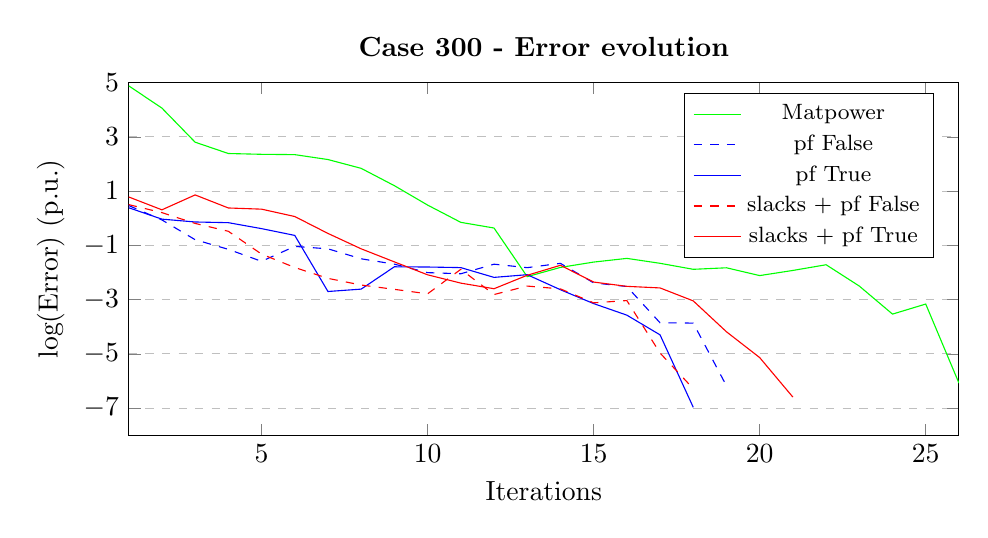
\begin{tikzpicture}
    \begin{semilogyaxis}[
        title={\textbf{Case 300 - Error evolution}},
        xlabel={Iterations},
        ylabel={log(Error) (p.u.)},
        width= \textwidth,
        height= 0.5\textwidth,
        xmin=1, xmax=26,
        ymin=1e-8, ymax=1e5,
        xtick={5,10,15,20,25},
        %ytick={1e-8,1e-6,1e-4,1e-2,1e0,1e2,1e4},
        log base 10 number format code/.code={\pgfmathprintnumber[fixed]{#1}},
        max space between ticks=20,
        legend pos=north east,
        ymajorgrids=true,
        grid style=dashed,
        scaled ticks=false,
        yticklabel style={/pgf/number format/sci},
        legend style={font=\footnotesize},        
    ]

    %Data for Matpower
    \addplot[
        color=green,
        mark=none,
        mark options={solid}
        ]
        coordinates {
            (1, 7.53E+04)
            (2, 1.14E+04)
            (3, 6.32E+02)
            (4, 2.42E+02)
            (5, 2.26E+02)
            (6, 2.20E+02)
            (7, 1.45E+02)
            (8, 6.87E+01)
            (9, 1.58E+01)
            (10, 3.05E+00)
            (11, 7.04E-01)
            (12, 4.35E-01)
            (13, 7.03E-03)
            (14, 1.54E-02)
            (15, 2.42E-02)
            (16, 3.31E-02)
            (17, 2.18E-02)
            (18, 1.31E-02)
            (19, 1.49E-02)
            (20, 7.69E-03)
            (21, 1.19E-02)
            (22, 1.93E-02)
            (23, 3.16E-03)
            (24, 2.93E-04)
            (25, 6.88E-04)
            (26, 8.43E-07)
            };
            \addlegendentry{Matpower}

    % Data for 'pf False' plotted with dashed lines
    \addplot[
        color=blue,
        dashed,
        mark=none,
        mark options={dashed}
        ]
        coordinates {
            (1, 2.936208787)
            (2, 0.863070361)
            (3, 0.161534637)
            (4, 0.071333199)
            (5, 0.025775797)
            (6, 0.091552775)
            (7, 0.07450434)
            (8, 0.031953639)
            (9, 0.020283202)
            (10, 0.009889533)
            (11, 0.008971603)
            (12, 0.020244771)
            (13, 0.015074886)
            (14, 0.021738874)
            (15, 0.004147349)
            (16, 0.003045018)
            (17, 0.000140213)
            (18, 0.000136692)
            (19, 6.64E-07)
            
        };
        \addlegendentry{pf False}

    % Data for 'pf True'
    \addplot[
        color=blue,
        mark=none,
        mark options={solid}
        ]
        coordinates {
            (1, 2.432229841)
            (2, 0.92458341)
            (3, 0.726214531)
            (4, 0.684812192)
            (5, 0.413152846)
            (6, 0.232583762)
            (7, 0.001993708)
            (8, 0.002440273)
            (9, 0.016226286)
            (10, 0.015922195)
            (11, 0.015141967)
            (12, 0.006602047)
            (13, 0.008294147)
            (14, 0.002318244)
            (15, 0.000714441)
            (16, 0.00026829)
            (17, 5.04E-05)
            (18, 1.08E-07)
            
        };
        \addlegendentry{pf True}

    %Data for slacks + pf False
    \addplot[
        color=red,
        mark=none,
        dashed,
        mark options={dashed}
        ]
        coordinates {
            (1, 3.167574855)
            (2, 1.603787928)
            (3, 0.642278168)
            (4, 0.329752885)
            (5, 0.047550026)
            (6, 0.015296491)
            (7, 0.006075237)
            (8, 0.003450498)
            (9, 0.002394262)
            (10, 0.00163828)
            (11, 0.013081511)
            (12, 0.001542913)
            (13, 0.003161681)
            (14, 0.002491171)
            (15, 0.00076242)
            (16, 0.000924757)
            (17, 1.08E-05) 
            (18, 5.23E-07)  
        };
        \addlegendentry{slacks + pf False}

         %Data for slacks + pf True'
    \addplot[
        color=red,
        mark=none,
        mark options={solid}
        ]
        coordinates {
            (1, 6.068166154)
            (2, 2.036464624)
            (3, 7.211447601)
            (4, 2.383818446)
            (5, 2.155179565)
            (6, 1.153516841)
            (7, 0.275017846)
            (8, 0.074454495)
            (9, 0.024604769)
            (10, 0.008204682)
            (11, 0.004061359)
            (12, 0.00252147)
            (13, 0.007900866)
            (14, 0.018418069)
            (15, 0.004443811)
            (16, 0.003086266)
            (17, 0.002698575)
            (18, 0.00089835)
            (19, 6.54E-05)
            (20, 7.33E-06)
            (21, 2.56E-07)
             
        };
        \addlegendentry{slacks + pf True}

    \end{semilogyaxis}
    \end{tikzpicture}
    \caption{Error evolution for the 300-bus system for different initialization options.}
    \label{fig:case300_error}
\end{figure}

The performance of the solver developed in this work outclasses the one of Matpower in this case. Considering that the solver is based on the same principles, this means that the GridCal modelled problem is better conditioned than the one modelled by Matpower,
which is why the solver has been developed in such an environment.

\subsubsection{Case GB}
Last case shown is a country-sized 2223-bus system that has been provided directly by Redeia, which models the Great Britain grid. Error evolutions are shown in Figure~\ref{fig:caseGB_error}.

%%%%%%%%%%%%%%%%%%%%%%%CASE GB


\begin{figure}[H]
    \centering
    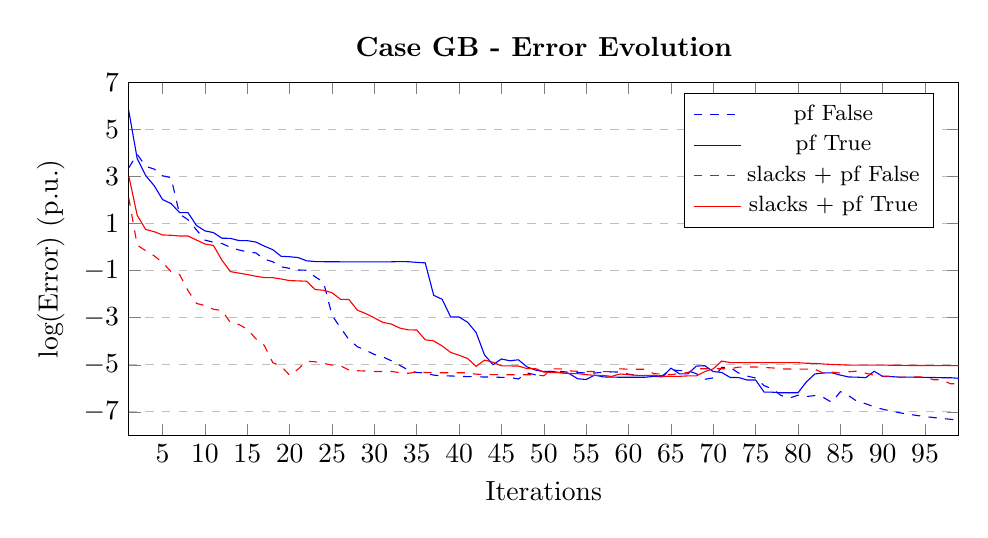
\begin{tikzpicture}
    \begin{semilogyaxis}[
        title={\textbf{Case GB - Error Evolution}},
        xlabel={Iterations},
        ylabel={log(Error) (p.u.)},
        width=\textwidth,
        height= 0.5\textwidth,
        xmin=1, xmax=99,
        ymin=1e-8, ymax=1e7,
        %xtick={10,20,30,40,50,60,70,80,90},
        %ytick={1e-8,1e-6,1e-4,1e-2,1e0,1e2,1e4,1e6},
        log base 10 number format code/.code={\pgfmathprintnumber[fixed]{#1}},
        max space between ticks=20,
        legend pos=north east,
        ymajorgrids=true,
        grid style=dashed,
        scaled ticks=false,
        yticklabel style={/pgf/number format/sci},
        legend style={font=\footnotesize},        
    ]

    % Data for 'pf False' plotted with dashed lines
    \addplot[
        color=blue,
        dashed,
        mark=none,
        mark options={dashed}
        ]
        coordinates {
            (1, 2352.813112)
            (2, 8928.483922)
            (3, 2734.583848)
            (4, 2091.219247)
            (5, 1083.581041)
            (6, 899.8106605)
            (7, 25.43791289)
            (8, 14.6163785)
            (9, 5.429096411)
            (10, 1.990894646)
            (11, 1.623204052)
            (12, 1.431413188)
            (13, 0.988402131)
            (14, 0.760754722)
            (15, 0.63180179)
            (16, 0.570487192)
            (17, 0.30913493)
            (18, 0.239603685)
            (19, 0.145910947)
            (20, 0.125213058)
            (21, 0.107168071)
            (22, 0.104320636)
            (23, 0.055052483)
            (24, 0.032543327)
            (25, 0.001261022)
            (26, 0.000374469)
            (27, 0.000116732)
            (28, 5.85E-05)
            (29, 4.10E-05)
            (30, 2.74E-05)
            (31, 2.17E-05)
            (32, 1.48E-05)
            (33, 9.42E-06)
            (34, 5.95E-06)
            (35, 4.68E-06)
            (36, 4.52E-06)
            (37, 3.63E-06)
            (38, 3.37E-06)
            (39, 3.35E-06)
            (40, 3.24E-06)
            (41, 3.12E-06)
            (42, 3.12E-06)
            (43, 3.01E-06)
            (44, 3.01E-06)
            (45, 2.92E-06)
            (46, 2.88E-06)
            (47, 2.49E-06)
            (48, 4.49E-06)
            (49, 3.78E-06)
            (50, 5.28E-06)
            (51, 5.26E-06)
            (52, 5.22E-06)
            (53, 4.78E-06)
            (54, 4.67E-06)
            (55, 4.50E-06)
            (56, 4.47E-06)
            (57, 4.81E-06)
            (58, 4.97E-06)
            (59, 4.94E-06)
            (60, 3.99E-06)
            (61, 3.50E-06)
            (62, 3.47E-06)
            (63, 3.46E-06)
            (64, 3.45E-06)
            (65, 6.08E-06)
            (66, 5.64E-06)
            (67, 5.53E-06)
            (68, 4.18E-06)
            (69, 2.42E-06)
            (70, 2.78E-06)
            (71, 7.69E-06)
            (72, 7.72E-06)
            (73, 4.43E-06)
            (74, 3.31E-06)
            (75, 2.74E-06)
            (76, 1.30E-06)
            (77, 9.35E-07)
            (78, 4.96E-07)
            (79, 3.88E-07)
            (80, 5.06E-07)
            (81, 4.48E-07)
            (82, 4.91E-07)
            (83, 4.07E-07)
            (84, 2.52E-07)
            (85, 7.20E-07)
            (86, 4.80E-07)
            (87, 2.75E-07)
            (88, 2.20E-07)
            (89, 1.63E-07)
            (90, 1.29E-07)
            (91, 1.07E-07)
            (92, 9.11E-08)
            (93, 7.94E-08)
            (94, 7.03E-08)
            (95, 6.31E-08)
            (96, 5.72E-08)
            (97, 5.23E-08)
            (98, 4.82E-08)
            (99, 4.47E-08)
            
        };
        \addlegendentry{pf False}

    % Data for 'pf True'
    \addplot[
        color=blue,
        mark=none,
        mark options={solid}
        ]
        coordinates {
            (1, 643178.5344)
            (2, 5900.292698)
            (3, 1106.700991)
            (4, 415.4098461)
            (5, 105.2807711)
            (6, 71.30182634)
            (7, 29.59955383)
            (8, 29.18531615)
            (9, 8.321889228)
            (10, 4.916244126)
            (11, 4.170715893)
            (12, 2.40607294)
            (13, 2.360678741)
            (14, 1.914702259)
            (15, 1.888603987)
            (16, 1.652948957)
            (17, 1.11008489)
            (18, 0.783511077)
            (19, 0.40843767)
            (20, 0.392203426)
            (21, 0.360863196)
            (22, 0.263150445)
            (23, 0.244530388)
            (24, 0.241226113)
            (25, 0.239070527)
            (26, 0.23851364)
            (27, 0.238473552)
            (28, 0.238473827)
            (29, 0.238469658)
            (30, 0.238469691)
            (31, 0.238469656)
            (32, 0.238469656)
            (33, 0.243976374)
            (34, 0.240570678)
            (35, 0.225341286)
            (36, 0.21569497)
            (37, 0.009008557)
            (38, 0.006080395)
            (39, 0.001082531)
            (40, 0.001072805)
            (41, 0.000644974)
            (42, 0.00023817)
            (43, 2.62E-05)
            (44, 1.01E-05)
            (45, 1.76E-05)
            (46, 1.48E-05)
            (47, 1.63E-05)
            (48, 8.21E-06)
            (49, 5.99E-06)
            (50, 5.03E-06)
            (51, 5.25E-06)
            (52, 4.56E-06)
            (53, 4.23E-06)
            (54, 2.54E-06)
            (55, 2.37E-06)
            (56, 3.64E-06)
            (57, 3.06E-06)
            (58, 2.98E-06)
            (59, 2.96E-06)
            (60, 2.96E-06)
            (61, 2.96E-06)
            (62, 2.96E-06)
            (63, 3.22E-06)
            (64, 3.06E-06)
            (65, 7.19E-06)
            (66, 4.12E-06)
            (67, 4.10E-06)
            (68, 8.77E-06)
            (69, 9.16E-06)
            (70, 5.15E-06)
            (71, 4.71E-06)
            (72, 2.89E-06)
            (73, 2.86E-06)
            (74, 2.26E-06)
            (75, 2.26E-06)
            (76, 6.93E-07)
            (77, 6.83E-07)
            (78, 6.47E-07)
            (79, 6.46E-07)
            (80, 6.44E-07)
            (81, 1.89E-06)
            (82, 4.08E-06)
            (83, 4.48E-06)
            (84, 4.56E-06)
            (85, 3.63E-06)
            (86, 3.03E-06)
            (87, 2.97E-06)
            (88, 2.83E-06)
            (89, 5.29E-06)
            (90, 3.20E-06)
            (91, 3.15E-06)
            (92, 2.98E-06)
            (93, 2.98E-06)
            (94, 2.96E-06)
            (95, 2.90E-06)
            (96, 2.88E-06)
            (97, 2.82E-06)
            (98, 2.82E-06)
            (99, 2.66E-06)
            
        };
        \addlegendentry{pf True}

    %Data for slacks + pf False
    \addplot[
        color=red,
        mark=none,
        dashed,
        mark options={dashed}
        ]
        coordinates {
            (1, 127.3283287)
            (2, 1.233341752)
            (3, 0.703699251)
            (4, 0.43017213)
            (5, 0.221907347)
            (6, 0.091207958)
            (7, 0.069120674)
            (8, 0.014185103)
            (9, 0.004054519)
            (10, 0.003296678)
            (11, 0.002286073)
            (12, 0.002032975)
            (13, 0.000624582)
            (14, 0.000515267)
            (15, 0.000326678)
            (16, 0.000128413)
            (17, 6.68E-05)
            (18, 1.23E-05)
            (19, 8.71E-06)
            (20, 3.57E-06)
            (21, 6.55E-06)
            (22, 1.41E-05)
            (23, 1.34E-05)
            (24, 1.14E-05)
            (25, 9.73E-06)
            (26, 9.10E-06)
            (27, 5.97E-06)
            (28, 5.58E-06)
            (29, 5.41E-06)
            (30, 5.20E-06)
            (31, 5.20E-06)
            (32, 5.20E-06)
            (33, 4.64E-06)
            (34, 4.34E-06)
            (35, 4.90E-06)
            (36, 4.69E-06)
            (37, 4.62E-06)
            (38, 4.59E-06)
            (39, 4.59E-06)
            (40, 4.58E-06)
            (41, 4.58E-06)
            (42, 3.99E-06)
            (43, 3.84E-06)
            (44, 3.81E-06)
            (45, 3.78E-06)
            (46, 3.76E-06)
            (47, 3.76E-06)
            (48, 3.76E-06)
            (49, 3.76E-06)
            (50, 3.41E-06)
            (51, 6.73E-06)
            (52, 6.72E-06)
            (53, 5.51E-06)
            (54, 5.27E-06)
            (55, 5.18E-06)
            (56, 5.15E-06)
            (57, 5.15E-06)
            (58, 5.15E-06)
            (59, 6.74E-06)
            (60, 6.46E-06)
            (61, 6.45E-06)
            (62, 6.45E-06)
            (63, 4.14E-06)
            (64, 4.12E-06)
            (65, 3.81E-06)
            (66, 4.22E-06)
            (67, 4.73E-06)
            (68, 6.83E-06)
            (69, 6.80E-06)
            (70, 6.80E-06)
            (71, 6.79E-06)
            (72, 6.79E-06)
            (73, 7.91E-06)
            (74, 8.06E-06)
            (75, 8.08E-06)
            (76, 7.69E-06)
            (77, 7.34E-06)
            (78, 6.66E-06)
            (79, 6.63E-06)
            (80, 6.60E-06)
            (81, 6.51E-06)
            (82, 6.49E-06)
            (83, 4.44E-06)
            (84, 4.87E-06)
            (85, 4.45E-06)
            (86, 5.02E-06)
            (87, 5.38E-06)
            (88, 4.37E-06)
            (89, 3.60E-06)
            (90, 3.32E-06)
            (91, 3.22E-06)
            (92, 2.94E-06)
            (93, 3.00E-06)
            (94, 3.03E-06)
            (95, 3.03E-06)
            (96, 2.31E-06)
            (97, 2.29E-06)
            (98, 1.56E-06)
            (99, 1.55E-06)
        };
        \addlegendentry{slacks + pf False}

         %Data for slacks + pf True'
    \addplot[
        color=red,
        mark=none,
        mark options={solid}
        ]
        coordinates {
        (1, 1091.229243)
        (2, 22.73981193)
        (3, 5.675467735)
        (4, 4.543233996)
        (5, 3.307131426)
        (6, 3.199128537)
        (7, 2.97460875)
        (8, 2.974125088)
        (9, 2.010558964)
        (10, 1.361382122)
        (11, 1.178734594)
        (12, 0.282020175)
        (13, 0.091440897)
        (14, 0.079111423)
        (15, 0.068560312)
        (16, 0.058161522)
        (17, 0.050883665)
        (18, 0.050581975)
        (19, 0.044334399)
        (20, 0.037813854)
        (21, 0.036831218)
        (22, 0.035580913)
        (23, 0.015837438)
        (24, 0.01468006)
        (25, 0.011571031)
        (26, 0.006077399)
        (27, 0.005921991)
        (28, 0.002086292)
        (29, 0.001488226)
        (30, 0.000981173)
        (31, 0.000635248)
        (32, 0.000539877)
        (33, 0.000363299)
        (34, 0.000305015)
        (35, 0.00030105)
        (36, 0.000115904)
        (37, 0.000103533)
        (38, 6.31E-05)
        (39, 3.36E-05)
        (40, 2.55E-05)
        (41, 1.85E-05)
        (42, 8.58E-06)
        (43, 1.58E-05)
        (44, 1.28E-05)
        (45, 9.00E-06)
        (46, 8.95E-06)
        (47, 8.83E-06)
        (48, 6.90E-06)
        (49, 6.90E-06)
        (50, 4.95E-06)
        (51, 4.63E-06)
        (52, 4.62E-06)
        (53, 4.25E-06)
        (54, 4.21E-06)
        (55, 3.80E-06)
        (56, 3.57E-06)
        (57, 3.53E-06)
        (58, 3.21E-06)
        (59, 4.06E-06)
        (60, 3.77E-06)
        (61, 3.57E-06)
        (62, 3.54E-06)
        (63, 3.52E-06)
        (64, 3.28E-06)
        (65, 3.23E-06)
        (66, 3.23E-06)
        (67, 3.37E-06)
        (68, 3.37E-06)
        (69, 5.13E-06)
        (70, 6.73E-06)
        (71, 1.44E-05)
        (72, 1.24E-05)
        (73, 1.24E-05)
        (74, 1.24E-05)
        (75, 1.24E-05)
        (76, 1.23E-05)
        (77, 1.23E-05)
        (78, 1.23E-05)
        (79, 1.23E-05)
        (80, 1.23E-05)
        (81, 1.16E-05)
        (82, 1.15E-05)
        (83, 1.08E-05)
        (84, 1.03E-05)
        (85, 1.00E-05)
        (86, 9.67E-06)
        (87, 9.66E-06)
        (88, 9.66E-06)
        (89, 9.66E-06)
        (90, 9.65E-06)
        (91, 9.57E-06)
        (92, 9.56E-06)
        (93, 9.34E-06)
        (94, 9.31E-06)
        (95, 9.28E-06)
        (96, 9.22E-06)
        (97, 9.17E-06)
        (98, 9.15E-06)
        (99, 9.15E-06)
             
        };
        \addlegendentry{slacks + pf True}
    \end{semilogyaxis}
    \end{tikzpicture}
    \caption{Error evolution for the Great Britain grid for different initialization options.}
    \label{fig:caseGB_error}
\end{figure}

In this case, there is no comparative with the Matpower solver since the data is stored in a file that can only be managed in GridCal, and the model is not public. The results show a really promising evolution for a real use case,
obtaining a low error in a few iterations. The slack initialization option can be preferred in this case, which is to be expected since it is a case that has not been tested before, and it might correspond 
to a difficult grid state (meaning the limits could be a bit strict, some generators/lines could be disabled or the load profile could be high).

Despite the good performance during the first steps, it stagnates when asking for lower tolerance values, a side effect of adding a lot of variables to the problem.


\subsection{Effect of tap variables control - Case IEEE14}

Once having seen the performance of the solver in some study cases, it is time to analyze the effect of the tap variables control. This control is a feature that allows the solver to manage the tap variables of the transformers in the grid, 
which are the ones that can be modified to control the voltage levels or the power transfer. This control can be done in two ways: by setting the tap variables as fixed variables or by setting them as optimization variables. The first option is the one 
that has been used in the previous subsections, and the second one is the one that is going to be tested in this one.

The grid used is the IEEE14 model grid \cite{dabbagchi1993power}, which is a 14-bus grid that includes transformers. Firstly, the error evolution is compared in Figures~\ref{fig:case14_error} and~\ref{fig:case14_tap_error} to see the effect of adding this tap variables. 

%%%% CASE14 normal

\begin{figure}[H]
    \centering
    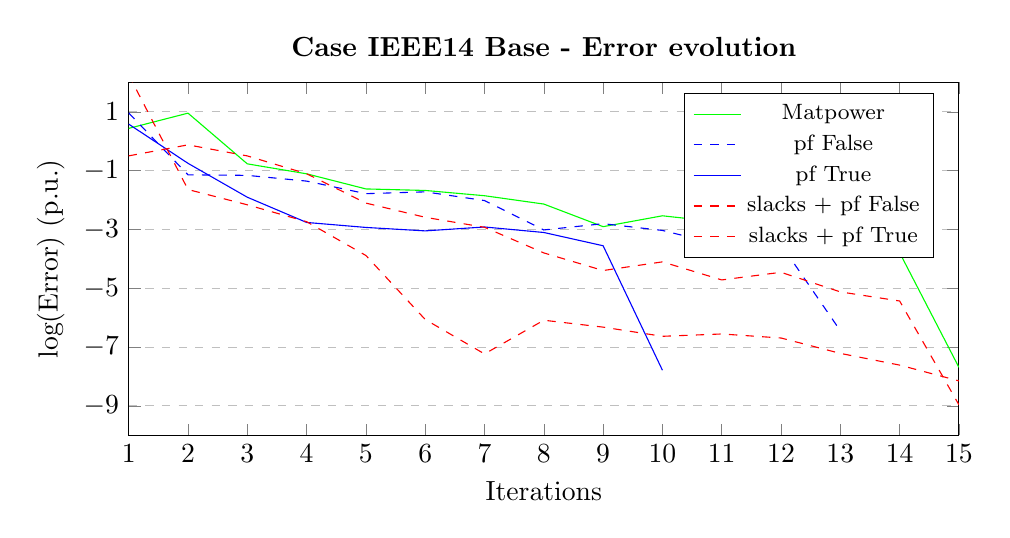
\begin{tikzpicture}
    \begin{semilogyaxis}[
        title={\textbf{Case IEEE14 Base - Error evolution}},
        xlabel={Iterations},
        ylabel={log(Error) (p.u.)},
        width=\textwidth,
        height= 0.5\textwidth,
        xmin=1, xmax=15,
        ymin=1e-10, ymax=1e2,
        log base 10 number format code/.code={\pgfmathprintnumber[fixed]{#1}},
        max space between ticks=20,
        legend pos=north east,
        ymajorgrids=true,
        grid style=dashed,
        scaled ticks=false,
        yticklabel style={/pgf/number format/sci},
        legend style={font=\footnotesize},        
    ]

    %Data for Matpower'
    \addplot[
        color=green,
        mark=none,
        mark options={solid}
        ]
        coordinates {
            (1, 2.75E+00)
            (2, 9.07E+00)
            (3, 1.71E-01)
            (4, 7.85E-02)
            (5, 2.40E-02)
            (6, 2.13E-02)
            (7, 1.41E-02)
            (8, 7.34E-03)
            (9, 1.25E-03)
            (10, 2.93E-03)
            (11, 1.76E-03)
            (12, 5.51E-04)
            (13, 6.50E-04)
            (14, 1.63E-04)
            (15, 2.05E-08)
        };
        \addlegendentry{Matpower}

    % Data for 'pf False' plotted with dashed lines
    \addplot[
        color=blue,
        dashed,
        mark=none,
        mark options={dashed}
        ]
        coordinates {
            (1, 9.213751716)
            (2, 0.072540437)
            (3, 0.069420068)
            (4, 0.044297854)
            (5, 0.016550251)
            (6, 0.019103711)
            (7, 0.009657606)
            (8, 0.000967572)
            (9, 0.001577085)
            (10, 0.000931124)
            (11, 0.000296858)
            (12, 0.000308507)
            (13, 3.61E-07)
            
        };
        \addlegendentry{pf False}

    % Data for 'pf True'
    \addplot[
        color=blue,
        mark=none,
        mark options={solid}
        ]
        coordinates {
            (1, 3.8416754)
            (2, 0.178257865)
            (3, 0.01254553)
            (4, 0.001738809)
            (5, 0.00117642)
            (6, 0.000898434)
            (7, 0.001219247)
            (8, 0.000792423)
            (9, 0.000280386)
            (10, 1.64E-08)
            
        };
        \addlegendentry{pf True}

    %Data for slacks + pf False
    \addplot[
        color=red,
        mark=none,
        dashed,
        mark options={dashed}
        ]
        coordinates {
            (1, 0.319744701)
            (2, 0.757329267)
            (3, 0.318402463)
            (4, 0.07900032)
            (5, 0.007922032)
            (6, 0.002602126)
            (7, 0.001190353)
            (8, 0.000160066)
            (9, 4.03E-05)
            (10, 7.94E-05)
            (11, 1.93E-05)
            (12, 3.51E-05)
            (13, 7.56E-06)
            (14, 3.71E-06)
            (15, 1.09E-09)
        };
        \addlegendentry{slacks + pf False}

    %Data for slacks + pf True
    \addplot[
        color=red,
        mark=none,
        dashed,
        mark options={dashed}
        ]
        coordinates {
            (1, 181.62441022700224)
            (2, 0.022897458206679974)
            (3, 0.006929041774338571)
            (4, 0.0018469169615173621)
            (5, 0.00013061962618515609)
            (6, 8.69767199952891e-07)
            (7, 5.8733757965589416e-08)
            (8, 8.222145107797376e-07)
            (9, 4.788624543636417e-07)
            (10, 2.3350350384465183e-07)
            (11, 2.8026613489491764e-07)
            (12, 2.0436953128261232e-07)
            (13, 6.124936153067041e-08)
            (14, 2.4486406772230067e-08)
            (15, 7.11319596670143e-09)
            (16, 7.80715019464817e-11)
        };
        \addlegendentry{slacks + pf True}
        
    \end{semilogyaxis}
    \end{tikzpicture}
    \caption{Error evolution for the Case IEEE14 for different initialization options.}
    \label{fig:case14_error}
\end{figure}


%%%% CASE14 taps

\begin{figure}[H]
    \centering
    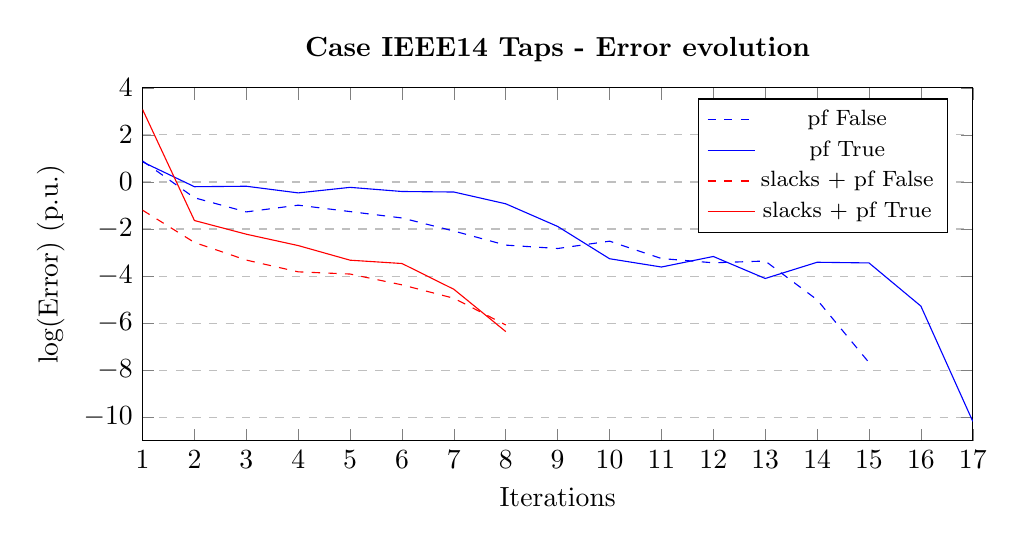
\begin{tikzpicture}
    \begin{semilogyaxis}[
        title={\textbf{Case IEEE14 Taps - Error evolution}},
        xlabel={Iterations},
        ylabel={log(Error) (p.u.)},
        width=\textwidth,
        height= 0.5\textwidth,
        xmin=1, xmax=17,
        ymin=1e-11, ymax=1e4,
        log base 10 number format code/.code={\pgfmathprintnumber[fixed]{#1}},
        max space between ticks=20,
        legend pos=north east,
        ymajorgrids=true,
        grid style=dashed,
        scaled ticks=false,
        yticklabel style={/pgf/number format/sci},
        legend style={font=\footnotesize},        
    ]

    % Data for 'pf False' plotted with dashed lines
    \addplot[
        color=blue,
        dashed,
        mark=none,
        mark options={dashed}
        ]
        coordinates {
            (1, 7.859900967)
            (2, 0.212772372)
            (3, 0.053400402)
            (4, 0.103219542)
            (5, 0.055136853)
            (6, 0.029458721)
            (7, 0.008210894)
            (8, 0.002070377)
            (9, 0.001485723)
            (10, 0.003043214)
            (11, 0.000556424)
            (12, 0.000366643)
            (13, 0.000436105)
            (14, 9.82E-06)
            (15, 2.10E-08)
        };
        \addlegendentry{pf False}

    % Data for 'pf True'
    \addplot[
        color=blue,
        mark=none,
        mark options={solid}
        ]
        coordinates {
            (1, 7.128524175)
            (2, 0.62936423)
            (3, 0.658239697)
            (4, 0.343270231)
            (5, 0.590285754)
            (6, 0.393917972)
            (7, 0.374122739)
            (8, 0.118023825)
            (9, 0.0128761)
            (10, 0.000546211)
            (11, 0.000242559)
            (12, 0.000679994)
            (13, 7.90E-05)
            (14, 0.000386629)
            (15, 0.00036193)
            (16, 5.28E-06)
            (17, 6.66E-11)
        };
        \addlegendentry{pf True}

    %Data for slacks + pf False
    \addplot[
        color=red,
        mark=none,
        dashed,
        mark options={dashed}
        ]
        coordinates {
            (1, 0.063322094)
            (2, 0.002683596)
            (3, 0.000477475)
            (4, 0.000151315)
            (5, 0.000122007)
            (6, 4.23E-05)
            (7, 1.14E-05)
            (8, 8.33E-07)
        };
        \addlegendentry{slacks + pf False}

         %Data for slacks + pf True'
    \addplot[
        color=red,
        mark=none,
        mark options={solid}
        ]
        coordinates {
            (1, 1210.715673)
            (2, 0.022978507)
            (3, 0.00602)
            (4, 0.001979625)
            (5, 0.000473052)
            (6, 0.000341739)
            (7, 2.74E-05)
            (8, 4.37E-07)
        };
        \addlegendentry{slacks + pf True}
    \end{semilogyaxis}
    \end{tikzpicture}
    \caption{Error evolution for the Case IEEE14 with tap variables for different initialization options.}
    \label{fig:case14_tap_error}
\end{figure}

There are two important remarks obtained from these error evolutions. Firstly, the case is solved in fewer iterations in the version of the solver developed in this project. Secondly, the usage of bound slacks improves convergence for the case with tap variables.
A more detailed analysis is done for the solution values for this case to analyze the impact of adding new optimization variables. For simplicity, the comparison will be made only for the cases with power flow initialization and without bound slacks, 
as they add to the cost function and the interest of this analysis is just testing the effect of using tap optimization.

Figures~\ref{fig:v_14} and~\ref{fig:gen_14} show the values of the solution for the bus voltages and generators. Note that there are no differences between the case solved with Matpower and the developed software.
The case with controlled tap variable has some slight differences, specially regarding the voltage magnitude. The impact in the generation is also noticeable for the reactive power generation, which has shifted mostly from generator 1 to generator 3.


\begin{figure}[H]
    \begin{minipage}{0.5\textwidth}
        \centering
        % Voltage Angles Plot
        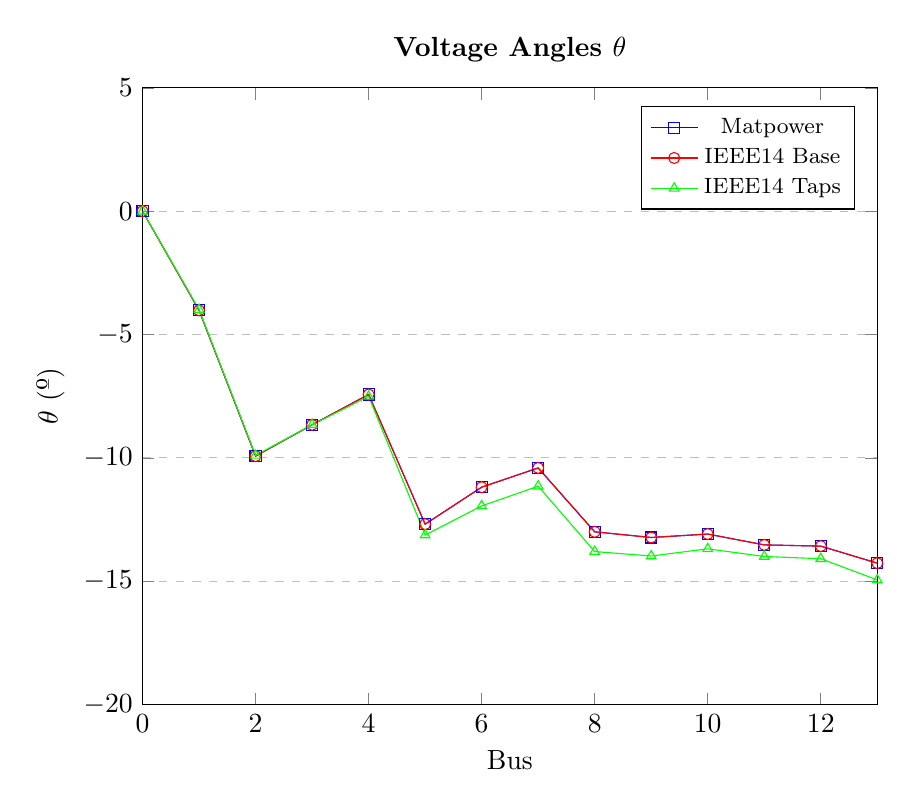
\begin{tikzpicture}
        \begin{axis}[
            title={\textbf{Voltage Angles $\theta$}},
            xlabel={Bus},
            ylabel={$\theta$ (º)},
            width = 0.9\textwidth,
            xmin=0, xmax=13,
            ymin=-20, ymax=5,
            xtick={0,2,4,6,8,10,12},
            ytick={-20,-15,-10,-5,0,5},
            legend pos=north east,
            legend style = {font = \footnotesize},
            ymajorgrids=true,
            grid style=dashed,
        ]

        \addplot[
            color=blue,
            mark=square,
            ]
            coordinates {
            (0,0.00) (1,-4.02) (2,-9.93) (3,-8.66) (4,-7.43) (5,-12.69) (6,-11.19) (7,-10.41) (8,-13.00) (9,-13.23) (10,-13.09) (11,-13.53) (12,-13.58) (13,-14.27)
            };
            \addlegendentry{Matpower}

        \addplot[
            color=red,
            mark=o,
            ]
            coordinates {
            (0,0.00) (1,-4.02) (2,-9.93) (3,-8.66) (4,-7.43) (5,-12.69) (6,-11.19) (7,-10.41) (8,-13.00) (9,-13.23) (10,-13.09) (11,-13.53) (12,-13.58) (13,-14.27)
            };
            \addlegendentry{IEEE14 Base}

        \addplot[
            color=green,
            mark=triangle,
            ]
            coordinates {
            (0,0.00) (1,-3.99) (2,-9.90) (3,-8.66) (4,-7.51) (5,-13.13) (6,-11.95) (7,-11.15) (8,-13.80) (9,-13.98) (10,-13.69) (11,-14.00) (12,-14.09) (13,-14.95)
            };
            \addlegendentry{IEEE14 Taps}
        \end{axis}
        \end{tikzpicture}
    \end{minipage}\hfill
    \begin{minipage}{0.5\textwidth}
        \centering
        % Voltage Magnitudes Plot
        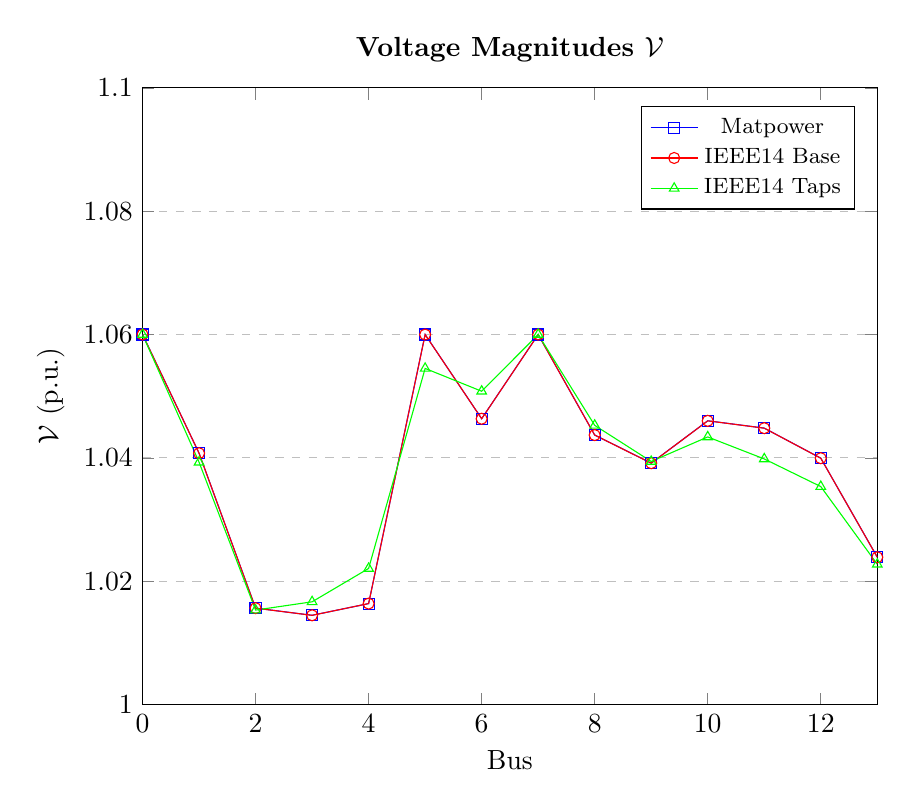
\begin{tikzpicture}
        \begin{axis}[
            title={\textbf{Voltage Magnitudes $\mathcal{V}$}},
            xlabel={Bus},
            ylabel={$\mathcal{V}$ (p.u.)},
            width=0.9\textwidth,
            xmin=0, xmax=13,
            ymin=1.0, ymax=1.1,
            xtick={0,2,4,6,8,10,12},
            ytick={1.00,1.02,1.04,1.06,1.08,1.10},
            legend pos=north east,
            legend style = {font = \footnotesize},
            ymajorgrids=true,
            grid style=dashed,
        ]

        \addplot[
            color=blue,
            mark=square,
            ]
            coordinates {
            (0,1.06000) (1,1.04075) (2,1.01563) (3,1.01446) (4,1.01636) (5,1.06000) (6,1.04635) (7,1.06000) (8,1.04370) (9,1.03914) (10,1.04601) (11,1.04482) (12,1.03995) (13,1.02389)
            };
            \addlegendentry{Matpower}

        \addplot[
            color=red,
            mark=o,
            ]
            coordinates {
            (0,1.06000) (1,1.04075) (2,1.01562) (3,1.01446) (4,1.01636) (5,1.05999) (6,1.04634) (7,1.05999) (8,1.04369) (9,1.03913) (10,1.04600) (11,1.04481) (12,1.03994) (13,1.02388)
            };
            \addlegendentry{IEEE14 Base}

        \addplot[
            color=green,
            mark=triangle,
            ]
            coordinates {
            (0,1.06000) (1,1.03929) (2,1.01531) (3,1.01665) (4,1.02206) (5,1.05450) (6,1.05080) (7,1.06000) (8,1.04527) (9,1.03941) (10,1.04339) (11,1.03982) (12,1.03534) (13,1.02274)
            };
            \addlegendentry{IEEE14 Taps}

        \end{axis}
        \end{tikzpicture}
    \end{minipage}
    \caption{Voltage comparison for the Case IEEE14 considering tap variables.}
    \label{fig:v_14}
\end{figure}


\begin{figure}[H]
    \begin{minipage}{0.5\textwidth}
        \centering

        % P (MW) Bar Graph
        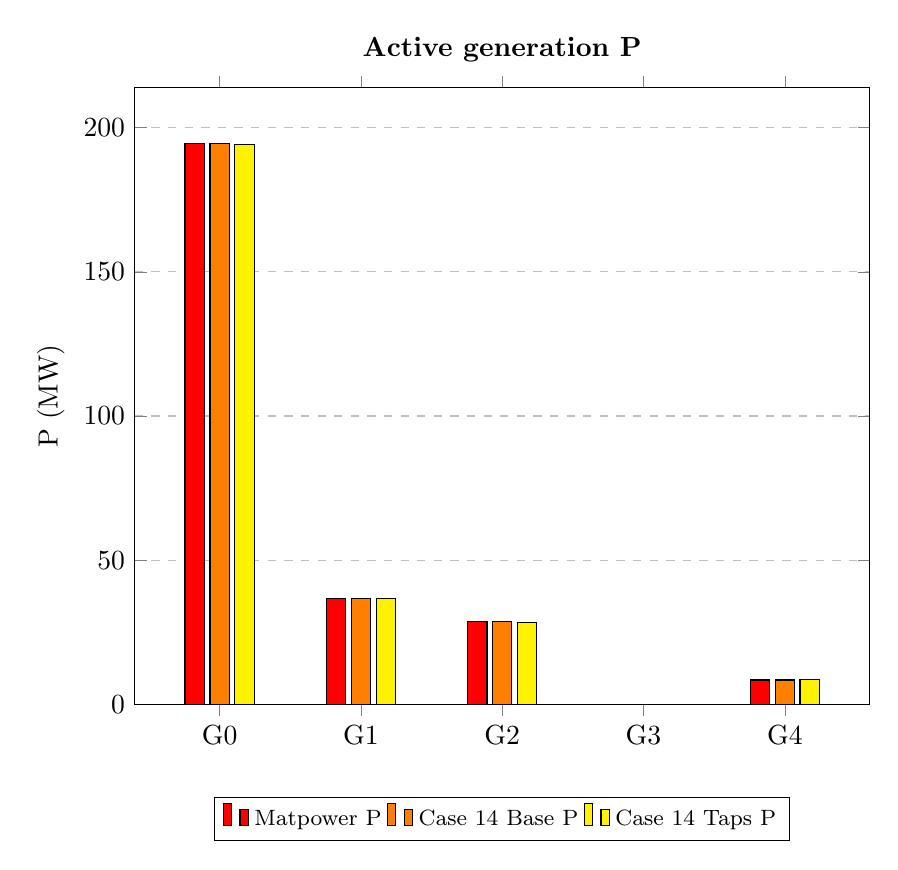
\begin{tikzpicture}
        \begin{axis}[
            title={\textbf{Active generation P}},
            ybar,
            enlarge x limits=0.15,
            ymin=0,
            width=0.9\textwidth,
            legend style={at={(0.5,-0.15)},
            anchor=north,legend columns=-1, font=\footnotesize},
            ylabel={P (MW)},
            symbolic x coords={G0,G1,G2,G3,G4},
            xtick=data,
            nodes near coords align={vertical},
            bar width=7pt,
            ymajorgrids,
            grid style=dashed,
        ]
        \addplot[fill=red]
            coordinates {(G0,194.33) (G1,36.72) (G2,28.74) (G3,0.00) (G4,8.50)};
        \addplot[fill=orange]
            coordinates {(G0,194.33) (G1,36.72) (G2,28.74) (G3,0.00) (G4,8.49)};
        \addplot[fill=yellow]
            coordinates {(G0,194.24) (G1,36.70) (G2,28.46) (G3,0.00) (G4,8.81)};
        
        \legend{Matpower P,Case 14 Base P,Case 14 Taps P}
        \end{axis}
        \end{tikzpicture}
    \end{minipage}\hfill
    \begin{minipage}{0.5\textwidth}
        \centering

        % Q (Mvar) Bar Graph
        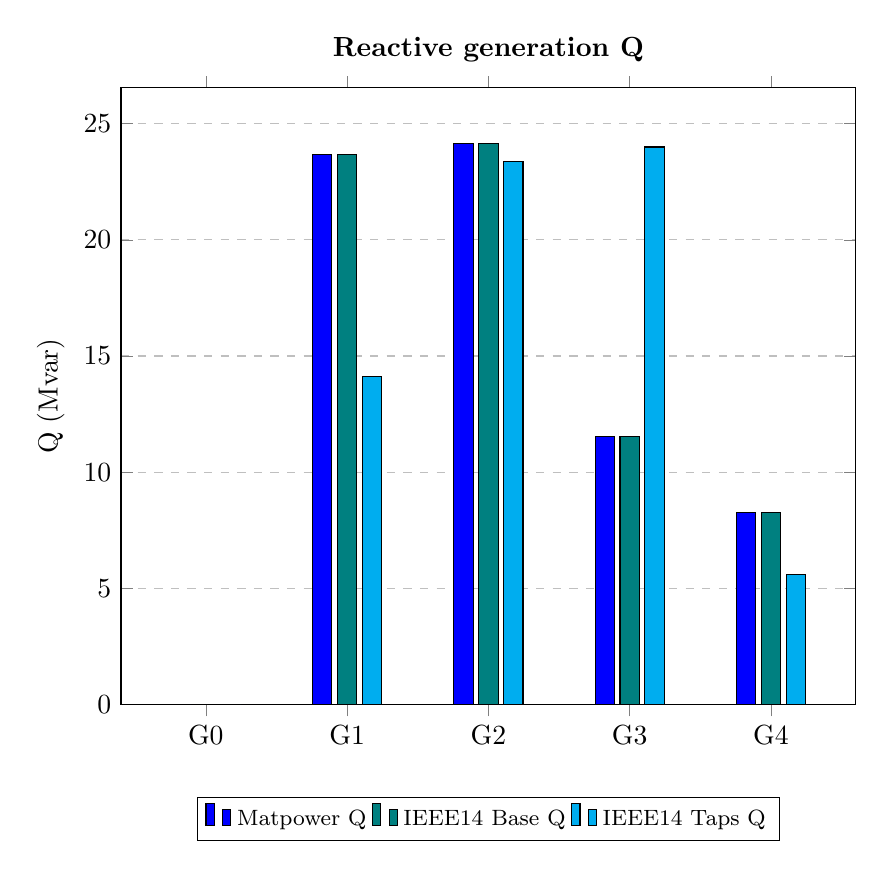
\begin{tikzpicture}
        \begin{axis}[
             title={\textbf{Reactive generation Q}},
            ybar,
            enlarge x limits=0.15,
            ymin=0,
            width=0.9\textwidth,
            legend style={at={(0.5,-0.15)},
            anchor=north,legend columns=-1, font=\footnotesize},
            ylabel={Q (Mvar)},
            symbolic x coords={G0,G1,G2,G3,G4},
            xtick=data,
            nodes near coords align={vertical},
            bar width=7pt,
            ymajorgrids,
            grid style = dashed,
        ]
        \addplot[fill=blue]
            coordinates {(G0,0.00) (G1,23.69) (G2,24.13) (G3,11.55) (G4,8.27)};
        \addplot[fill=teal]
            coordinates {(G0,0.01) (G1,23.68) (G2,24.13) (G3,11.54) (G4,8.27)};
        \addplot[fill=cyan]
            coordinates {(G0,0.00) (G1,14.11) (G2,23.37) (G3,24.00) (G4,5.60)};
        
        \legend{Matpower Q, IEEE14 Base Q, IEEE14 Taps Q}
        \end{axis}
        \end{tikzpicture}
\end{minipage}
    \caption{Generation comparison for Case IEEE14.}
    \label{fig:gen_14}
\end{figure}

Table~\ref{tab:tap_setpoints} shows the setpoints for the tap variables of the transformers in the grid as obtained with the solver developed. Note that the transformers that only have one variable controlled have a $N/C$ (Non-Controlled) as a solution.

\begin{table}[H]
    \centering
    \caption{Tap variable setpoints for the transformers of the corresponding branches in IEEE14.}
    \begin{tabular}{lcc}
    \hline
    \textbf{Controlled trafos} & \textbf{m\_p (p.u)} & \textbf{$\tau$ (º)} \\ \hline\hline
    Branch 17                  & 0.965876            & 0.754872          \\ 
    Branch 18                  & N/C                 & 1.365530          \\ 
    Branch 19                  & 0.974728            & N/C                \\ \hline
    \end{tabular}
    
    \label{tab:tap_setpoints}
\end{table}

The important result is shown in Table~\ref{tab:costs_tap}, which shows the impact of being able to control the tap variables setpoints in the cost of operation. Of course, this impact may not seem big in this case, representing
a reduction of cost of only 0.03\%. However, this result has only considered a small grid, without using properly modelled generation costs, and only controlling three transformers. And still, considering the total expenses of a country-sized grid as well as this result
being an instant photo of a given grid state, it can translate in substantial savings in the long-term. 

\begin{table}[H]
    \centering
    \caption{Comparison of costs between different cases.}
    \begin{tabular}{lccc}
    \hline
                          & \textbf{Matpower} & \textbf{Case 14 Base} & \textbf{Case 14 Taps} \\ \hline\hline
    \textbf{Cost (€/MWh)} & 8081.53           & 8081.53                  & 8078.85               \\ \hline
    \end{tabular}
    \label{tab:costs_tap}
    \end{table}
    

\subsection{Effect of reactive control}

Using the same base case, now the test is performed over the reactive power control. The limit is set as a maximum of a power factor of 0.8, which is translated to a maximum reactive power generation of 75\% of the active power generation.
The constraint is applied with respect to the absolute value of Q, meaning this constraint applies to both the injection and consumption of reactive power. Figure~\ref{fig:ctQ_V} shows the effect in the voltage values. There is a noticeable drop in magnitude in some of the buses.

\begin{figure}[!htb]
    \begin{minipage}{0.5\textwidth}
        \centering
        % Voltage Angles Plot
        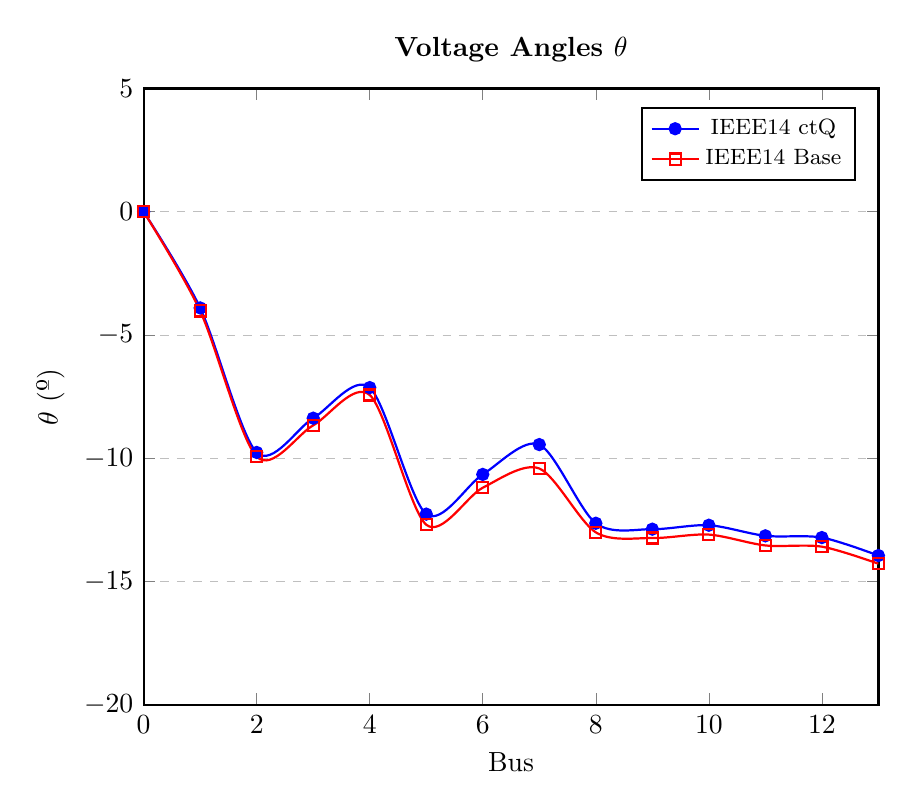
\begin{tikzpicture}
        \begin{axis}[
            title={\textbf{Voltage Angles $\theta$}},
            width=0.9\textwidth,
            xlabel={Bus},
            ylabel={$\theta$ (º)},
            xmin=0, xmax=13,
            ymin=-20, ymax=5,
            legend pos=north east,
            ymajorgrids=true,
            grid style=dashed,
            thick,
            legend style={font=\footnotesize},
        ]
        % Case 14 ctQ - Va
        \addplot[
            color=blue,
            mark=*,
            smooth,
            ]
            coordinates {
            (0,0.00) (1,-3.90) (2,-9.76) (3,-8.37) (4,-7.13) (5,-12.26) (6,-10.65) (7,-9.44) (8,-12.63) (9,-12.87) (10,-12.71) (11,-13.14) (12,-13.21) (13,-13.94)
            };
            \addlegendentry{IEEE14 ctQ}

        % Case 14 Base - Theta
        \addplot[
            color=red,
            mark=square,
            smooth,
            ]
            coordinates {
            (0,0.00) (1,-4.02) (2,-9.93) (3,-8.66) (4,-7.43) (5,-12.69) (6,-11.19) (7,-10.41) (8,-13.00) (9,-13.23) (10,-13.09) (11,-13.53) (12,-13.58) (13,-14.27)
            };
            \addlegendentry{IEEE14 Base}
        \end{axis}
        \end{tikzpicture}
    \end{minipage}\hfill
    \begin{minipage}{0.5\textwidth}
        \centering
        % Voltage Magnitudes Plot
        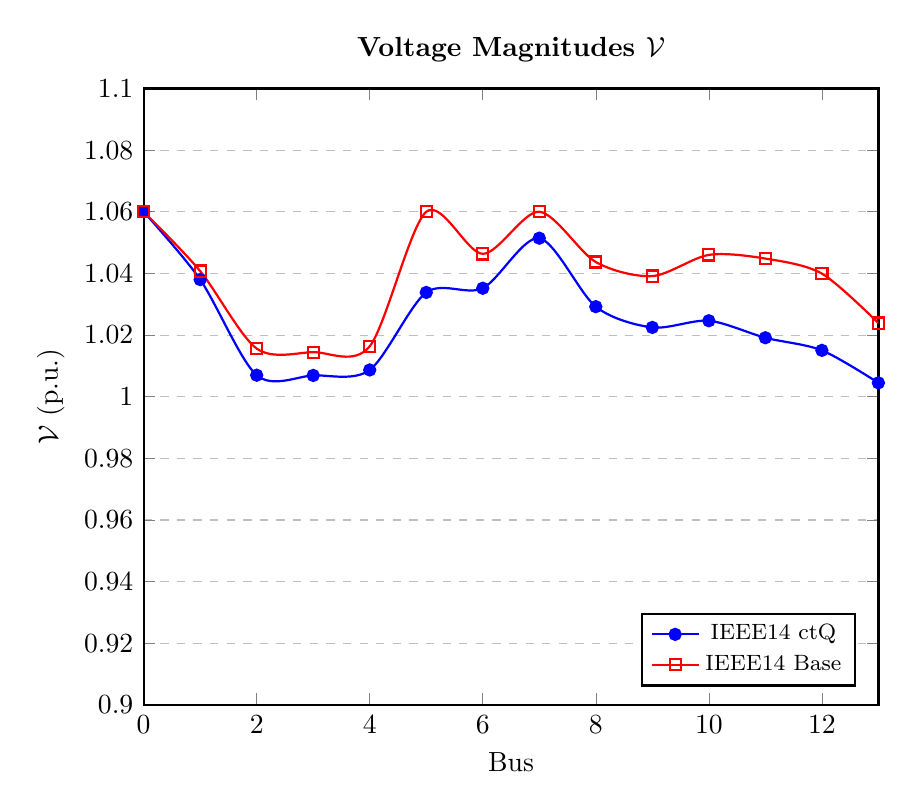
\begin{tikzpicture}
        \begin{axis}[
            title={\textbf{Voltage Magnitudes $\mathcal{V}$}},
            width=0.9\textwidth,
            xlabel={Bus},
            ylabel={$\mathcal{V}$ (p.u.)},
            xmin=0, xmax=13,
            ymin=0.9, ymax=1.1,
            legend pos=south east,
            ymajorgrids=true,
            grid style=dashed,
            thick,
            legend style={font=\footnotesize},
        ]

        % Case 14 ctQ - Vm
        \addplot[
            color=blue,
            mark=*,
            smooth,
            ]
            coordinates {
            (0,1.06000) (1,1.03800) (2,1.00698) (3,1.00691) (4,1.00868) (5,1.03382) (6,1.03519) (7,1.05143) (8,1.02921) (9,1.02248) (10,1.02464) (11,1.01913) (12,1.01504) (13,1.00450)
            };
            \addlegendentry{IEEE14 ctQ}

        % Case 14 Base - v
        \addplot[
            color=red,
            mark=square,
            smooth,
            ]
            coordinates {
            (0,1.06000) (1,1.04075) (2,1.01562) (3,1.01446) (4,1.01636) (5,1.05999) (6,1.04634) (7,1.05999) (8,1.04369) (9,1.03913) (10,1.04600) (11,1.04481) (12,1.03994) (13,1.02388)
            };
            \addlegendentry{IEEE14 Base}
        \end{axis}
        \end{tikzpicture}
    \end{minipage}
    \caption{Voltage comparison for the Case IEEE14 with and without reactive control.}
    \label{fig:ctQ_V}
\end{figure}


In Figure~\ref{fig:ctQ_gen}, it can be seen that generator 2, which previously had a reactive generation of 24.12 Mvar, now has a generation of 20.96 Mvar, which corresponds exactly to the 75\% of the active power generation.
This generator being at its limit for reactive power generation means the other generator have to contribute to reactive generation, impacting the voltage levels in the grid.

\begin{figure}[H]
    \centering
    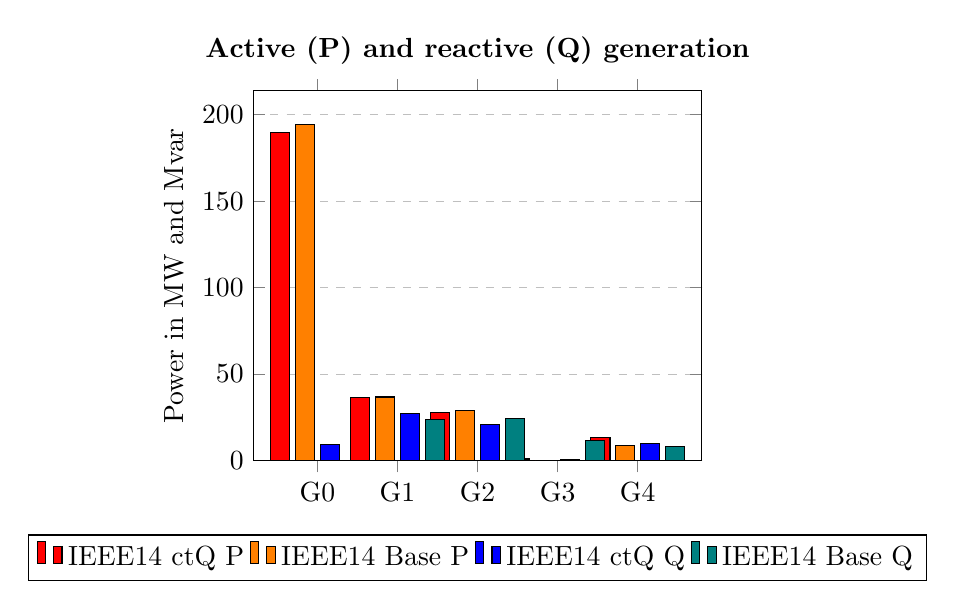
\begin{tikzpicture}
    \begin{axis}[
        title={\textbf{Active (P) and reactive (Q) generation}},
        ybar,
        enlarge x limits=0.2,
        ymin=0,
        width=0.6\textwidth,
        legend style={at={(0.5,-0.2)},
        anchor=north,legend columns=-1},
        ylabel={Power in MW and Mvar},
        symbolic x coords={G0, G1, G2, G3, G4},
        xtick=data,
        nodes near coords align={vertical},
        bar width=7pt,
        ymajorgrids,
        grid style=dashed,
    ]

    \addplot[fill=red] coordinates {(G0,189.83) (G1,36.28) (G2,27.95) (G3,0.85) (G4,13.10)};
    \addplot[fill=orange] coordinates {(G0,194.33) (G1,36.72) (G2,28.74) (G3,0.00) (G4,8.49)};
    \addplot[fill=blue] coordinates {(G0,9.26) (G1,27.21) (G2,20.96) (G3,0.64) (G4,9.83)};
    \addplot[fill=teal] coordinates {(G0,0.01) (G1,23.68) (G2,24.13) (G3,11.54) (G4,8.27)};

    \legend{IEEE14 ctQ P, IEEE14 Base P, IEEE14 ctQ Q, IEEE14 Base Q}
    \end{axis}
    \end{tikzpicture}
    \caption{Generation comparison for the Case IEEE14 with and without reactive control.} 
    \label{fig:ctQ_gen}
\end{figure}

The effect of this constraint can be seen in the cost value of the simulation. Table~\ref{tab:ctQ_cost} shows an increase of around 0.075\% in the cost of operation, which again can be significant in a bigger grid.

\begin{table}[H]
    \centering
    \caption{Cost for Case IEEE14 with Q control.}
    \begin{tabular}{lcc}
    \hline
     & {\textbf{IEEE14 Base}}& {\textbf{IEEE14 ctQ}}\\ \hline\hline
    \textbf{Cost (€/MWh)} & 8081.53 & 8087.82 \\ \hline
    \end{tabular}
    \label{tab:ctQ_cost}
\end{table}

\subsection{DC link and dual price study}

The following study is performed over a small grid with two islands of three buses each. Both of them have the same configuration and elements, but their generators will have different costs profiles as follows:

\begin{equation}
    \begin{split}
        c_{g1.0}(P_{g1.0}) &= 1 \cdot P_{g1.0} + 2 \cdot P_{g1.0}^2 \\
        c_{g1.1}(P_{g1.1}) &= 1 \cdot P_{g1.1} + 3 \cdot P_{g1.1}^2 \\
        c_{g2.0}(P_{g2.0}) &= 1 \cdot P_{g2.0} + 1.5 \cdot P_{g2.0}^2 \\
        c_{g2.1}(P_{g2.1}) &= 1 \cdot P_{g2.1} + 1 \cdot P_{g2.1}^2
    \end{split}
\end{equation}

The grid is firstly tested without interconnection, obtaining the results for each island isolated. Then, a lossless DC link is added between the two islands. In Figure~\ref{fig:island_gen}, 
the comparison between the generation profiles can be seen.

\begin{figure}[H]
    \centering
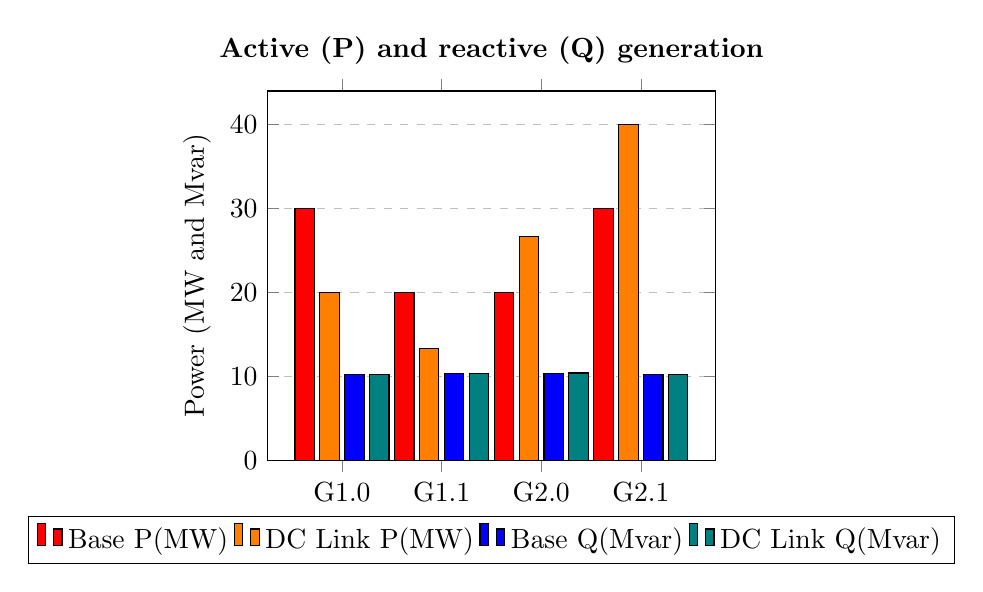
\begin{tikzpicture}
    \begin{axis}[
        title={\textbf{Active (P) and reactive (Q) generation}},
        ybar,
        enlarge x limits=0.25,
        ymin=0,
        width=0.6\textwidth,
        legend style={at={(0.5,-0.15)},
        anchor=north,legend columns=-1},
        ylabel={Power (MW and Mvar)},
        symbolic x coords={G1.0,G1.1,G2.0,G2.1},
        xtick=data,
        nodes near coords align={vertical},
        bar width=7pt,
        ymajorgrids,
        grid style=dashed,
    ]
    \addplot[fill=red] coordinates {(G1.0,30.01) (G1.1,20.01) (G2.0,20.01) (G2.1,30.01)};
    \addplot[fill=orange] coordinates {(G1.0,20.01) (G1.1,13.34) (G2.0,26.67) (G2.1,40.01)};
    \addplot[fill=blue] coordinates {(G1.0,10.26) (G1.1,10.35) (G2.0,10.36) (G2.1,10.25)};
    \addplot[fill=teal] coordinates {(G1.0,10.25) (G1.1,10.39) (G2.0,10.42) (G2.1,10.25)};

    \legend{Base P(MW), DC Link P(MW), Base Q(Mvar), DC Link Q(Mvar)}
    \end{axis}
    \end{tikzpicture}
    \caption{Generation comparison for the island case with and without DC link.}
    \label{fig:island_gen}
\end{figure}

As expected, after both grids are connected, the generators of the second island become prevalent as their prices are lower than the first island, and the power is transferred through this DC link with a total power
of $P_{DC} = 16.67 \text{MW}$. The interconnection has a great impact in the dual price as seen in Figure~\ref{fig:dual_price}.

\begin{figure}[H]
    \centering
    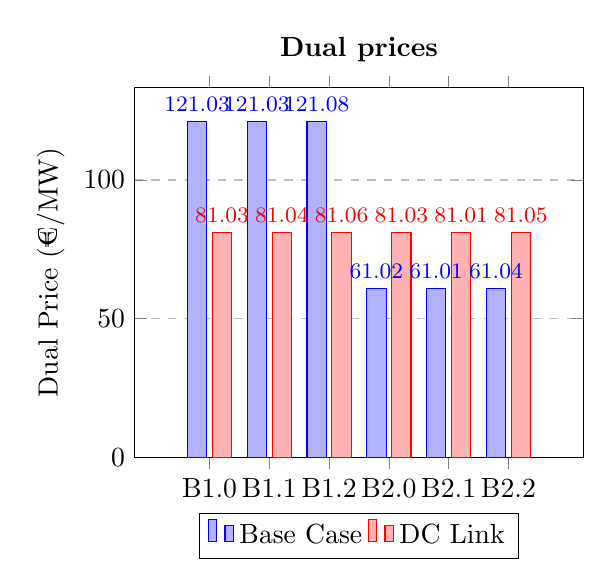
\begin{tikzpicture}
    \begin{axis}[
        title={\textbf{Dual prices}},
        ybar,
        enlarge x limits=0.25,
        ymin=0,
        width=0.6\textwidth,
        legend style={at={(0.5,-0.15)},
        anchor=north,legend columns=-1},
        ylabel={Dual Price (€/MW)},
        symbolic x coords={B1.0,B1.1,B1.2,B2.0,B2.1,B2.2},
        xtick=data,
        nodes near coords,
        nodes near coords align={vertical},
        nodes near coords style={font=\footnotesize},
        bar width=7pt,
        ymajorgrids,
        grid style=dashed,
    ]
    \addplot coordinates {(B1.0,121.027) (B1.1,121.034) (B1.2,121.081) (B2.0,61.017) (B2.1,61.013) (B2.2,61.041)};
    \addplot coordinates {(B1.0,81.025) (B1.1,81.035) (B1.2,81.064) (B2.0,81.025) (B2.1,81.012) (B2.2,81.052)};

    \legend{Base Case, DC Link}
    \end{axis}
    \end{tikzpicture}

    \caption{Dual price comparison for the case with and without DC link.}
    \label{fig:dual_price}
\end{figure}

These results are really important to understand the meaning of the dual price, which for the optimization problem are equal to the value of the equality multipliers associated to the nodal power balance
of each bus. These values indicate the rate of increase in cost that would be caused by demanding an additional infinitesimal amount of power at that bus. 
The following calculations can be done to check which is the cost of generating an additional MW of power per generation, using their cost function and the obtained setpoint from the optimization solution:

\begin{equation}
    \begin{split}
        \frac{\partial c_{g1.0}}{\partial P_{g1.0}}_{Base} & = 1 + 4 \cdot P_{g1.0} = 1 + 4 \cdot 30.0067 = 121.027 \\
        \frac{\partial c_{g1.1}}{\partial P_{g1.1}}_{Base} & = 1 + 6 \cdot P_{g1.1} = 1 + 6 \cdot 20.0056 = 121.034 \\
        \frac{\partial c_{g2.0}}{\partial P_{g2.0}}_{Base} & = 1 + 3 \cdot P_{g2.0} = 1 + 3 \cdot 20.0056 = 61.017 \\
        \frac{\partial c_{g2.1}}{\partial P_{g2.1}}_{Base} & = 1 + 2 \cdot P_{g2.1} = 1 + 2 \cdot 30.0067 = 61.013 \\
    \end{split}
\end{equation}

\begin{equation}
    \begin{split}
        \frac{\partial c_{g1.0}}{\partial P_{g1.0}}_{DC} & = 1 + 4 \cdot P_{g1.0} = 1 + 4 \cdot 20.0062 = 81.025 \\
        \frac{\partial c_{g1.1}}{\partial P_{g1.1}}_{DC} & = 1 + 6 \cdot P_{g1.1} = 1 + 6 \cdot 13.3392 = 81.035 \\
        \frac{\partial c_{g2.0}}{\partial P_{g2.0}}_{DC} & = 1 + 3 \cdot P_{g2.0} = 1 + 3 \cdot 26.6750 = 81.025 \\
        \frac{\partial c_{g2.1}}{\partial P_{g2.1}}_{DC} & = 1 + 2 \cdot P_{g2.1} = 1 + 2 \cdot 40.0057 = 81.012 \\
    \end{split}
\end{equation}

As it can be seen, the values of dual prices for buses with generation are equal to the derivative of those generators connected. For buses with no generation, the price is slightly above since it has to 
account for the additional power injected due to the losses during the power transfer.

Finally, the cost of operation has obviously been reduced after connecting both islands as seen in Table~\ref{tab:DC_cost}. The difference is significant, 
representing a reduction of 11.5\% in the cost of operation. This example shows the economical benefit of having an interconnection to a neighboring grid as the INELFE interconnection between 
Spain and France, apart from the technical benefits in terms of frequency stability, power support during faults, etc. 

\begin{table}[H]
    \centering
    \caption{Costs for Case 2 islands.}
    \begin{tabular}{lcc}
    \hline
     & {\textbf{Base Case 2 islands}}& {\textbf{2 islands + DC link}}\\ \hline\hline
    \textbf{Cost (€/MWh)} & 4602.23 & 4102.12 \\\hline
    \end{tabular}
    \label{tab:DC_cost}
\end{table}


\subsection{Runtime comparison}

Lastly, the execution times of all the cases with each different initialization combination have been measured. All measurements have been reproduced in the same conditions, repeating 5 times each execution to have a larger sample size, although
all the values had low deviation. Results are shown in Figures~\ref{fig:runtime} and~\ref{fig:GBruntime}, separating the larger case for better visualization. 

Overall, the solver seems to be on the same level of performance as Matpower in the cases where a comparison could be made. For smaller cases, Matpower has a slight advantage, while for bigger cases the initialization with a power flow solution
greatly improves the performance of the solver. The slack initialization is slower in most of the cases as expected, but in some cases it performs at the same level as the power flow initialization with no slacks. Bear in mind that this option is not
expected to be used for improved speed, rather for improved convergence.

An important remark to be made is that the power flow execution time is not included in the runtime of the solver, as it is assumed that the user would be able to calculate it once with the built-in power flow
solver, and then use it directly for all the desired studies. Another remark is that this comparison is made with the Python adaptation of Matpower, while the original implementation runs in Matlab/Octave and should be quicker.



\begin{figure}[!htb]
    \centering
    \begin{tikzpicture}
        \begin{axis}[
            ybar,
            ymin=0,
            bar width=7pt,
            width=\textwidth,
            height=0.4\textheight,
            enlarge x limits=0.25,
            legend style={at={(0.5,-0.3)},
                anchor=north,legend columns=-1},
            ylabel={Runtime (s)},
            symbolic x coords={Case 9, IEEE14, IEEE14 Taps, Pegase89, IEEE300, Case GB},
            xtick=data,
            nodes near coords align={vertical},
            x tick label style={rotate=45, anchor=east},
            legend style={font=\footnotesize},
            ymajorgrids,
            grid style=dashed,
        ]

        % MATPOWER
        \addplot[fill=green] coordinates {(Case 9,0.30) (IEEE14,0.39) (IEEE14 Taps, 0) (Pegase89,0.75) (IEEE300,1.38)};
        
        % PowerFlow
        \addplot[fill=red] coordinates {(Case 9,0.52) (IEEE14,0.42) (IEEE14 Taps,0.80) (Pegase89,0.66) (IEEE300,0.93)};
        
        % No PowerFlow
        \addplot[fill=orange] coordinates {(Case 9,0.50) (IEEE14,0.51) (IEEE14 Taps,0.83) (Pegase89,1.02) (IEEE300,1.03)};
        
        % PowerFlow + slacks
        \addplot[fill=blue] coordinates {(Case 9,0.65) (IEEE14,0.64) (IEEE14 Taps,0.92) (Pegase89,0.64) (IEEE300,1.60)};
        
        % No PowerFlow + slacks
        \addplot[fill=cyan] coordinates {(Case 9,0.65) (IEEE14,0.67) (IEEE14 Taps,0.78) (Pegase89,2.18) (IEEE300,1.22)};

        \legend{MATPOWER,PowerFlow,No PowerFlow,PowerFlow + slacks,No PowerFlow + slacks}
        \end{axis}
    \end{tikzpicture}
    \caption{Runtime comparison for different cases.}
    \label{fig:runtime}
\end{figure}


\begin{figure}[!htb]
    \centering
    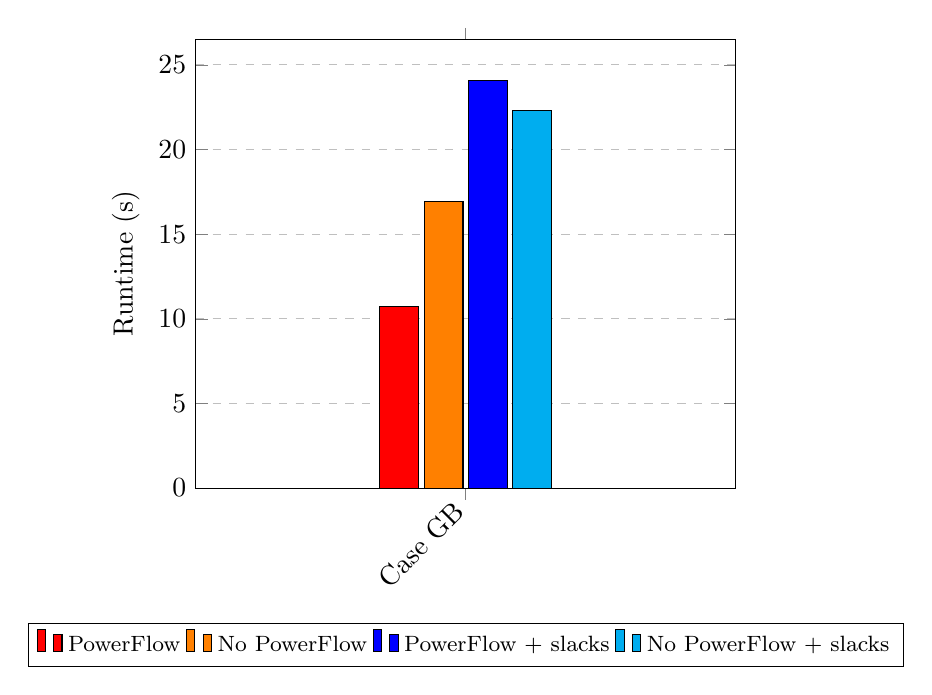
\begin{tikzpicture}
        \begin{axis}[
            ybar,
            enlarge x limits=0.5,
            ymin=0,
            bar width=14pt,
            legend style={at={(0.5,-0.3)},
            anchor=north,legend columns=-1},
            ylabel={Runtime (s)},
            symbolic x coords={Case GB},
            xtick=data,
            nodes near coords align={vertical},
            x tick label style={rotate=45, anchor=east},
            legend style={font=\footnotesize},
            ymajorgrids,
            grid style=dashed,
        ]
        % PowerFlow
        \addplot[fill=red] coordinates {(Case GB,10.75)};
        
        % No PowerFlow
        \addplot[fill=orange] coordinates {(Case GB,16.92)};
        
        % PowerFlow + slacks
        \addplot[fill=blue] coordinates {(Case GB,24.08)};
        
        % No PowerFlow + slacks
        \addplot[fill=cyan] coordinates {(Case GB,22.30)};

        \legend{PowerFlow,No PowerFlow,PowerFlow + slacks,No PowerFlow + slacks}
        \end{axis}
    \end{tikzpicture}
    \caption{Runtime comparison for the GB case.}
    \label{fig:GBruntime}
\end{figure}
